\documentclass[tikz,border=4mm]{standalone}
\usetikzlibrary{positioning, arrows.meta, fit, calc, backgrounds}

\begin{document}
\sffamily\fontsize{8pt}{10pt}\selectfont
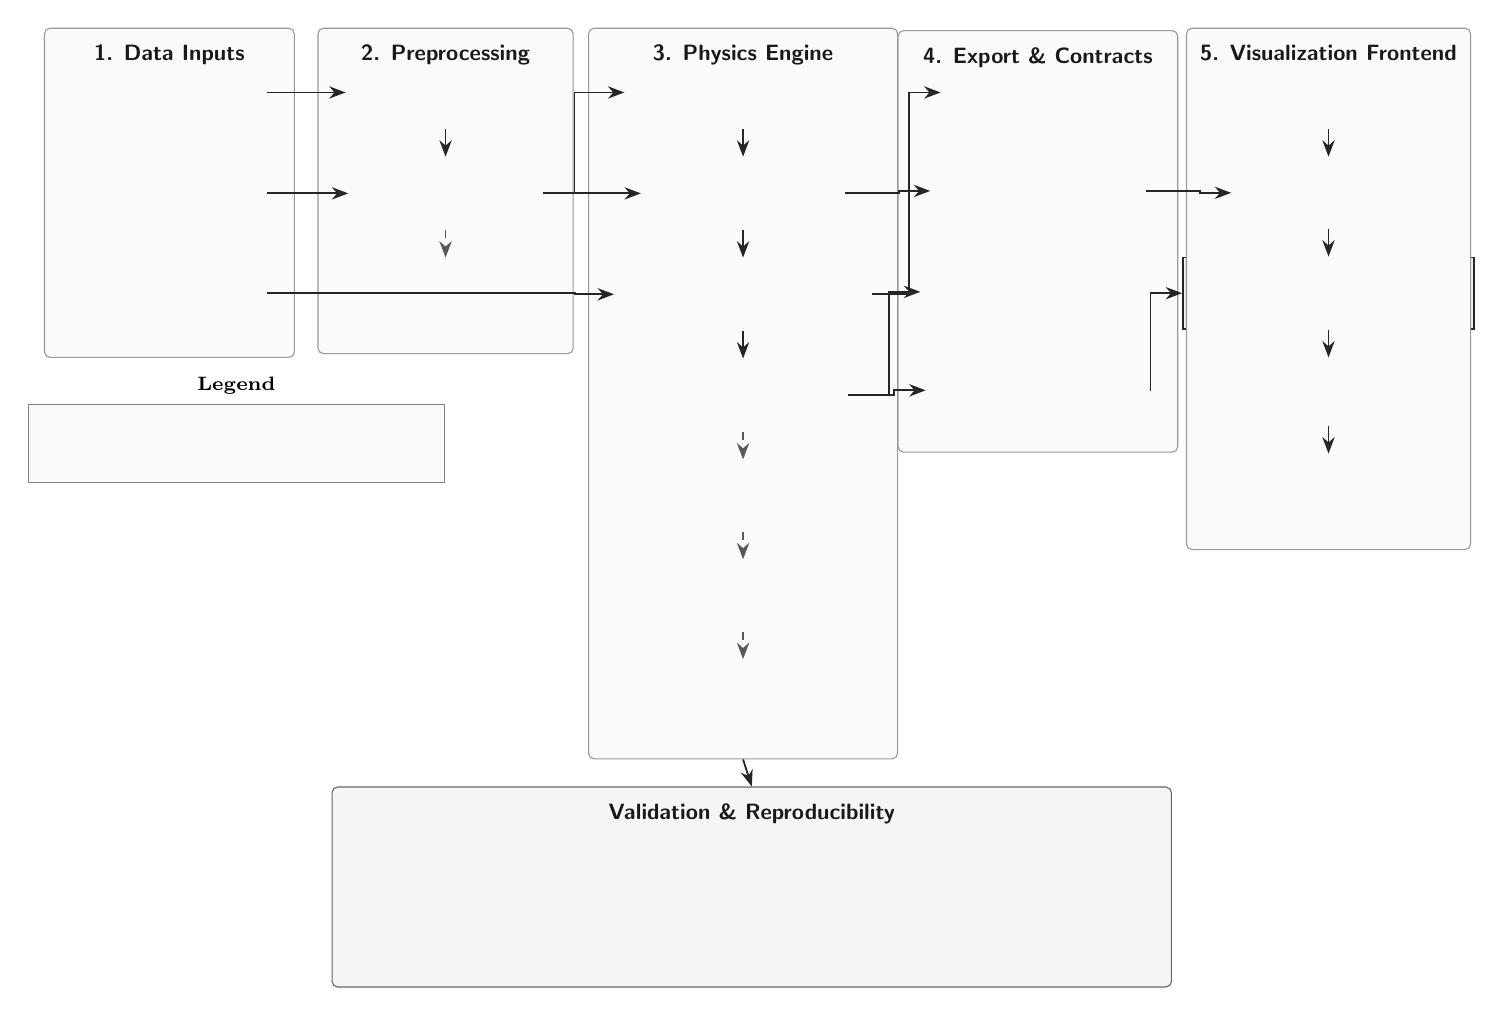
\begin{tikzpicture}[
    >=Stealth,
    node distance=6mm and 8mm,
    % Box Styles (Grayscale-safe, IEEE publication standard)
    layerbg/.style={
        draw=black!40,
        fill=black!2,
        rounded corners=2pt,
        inner sep=3.5mm
    },
    layertitle/.style={
        font=\sffamily\fontsize{8.5pt}{10pt}\bfseries,
        text=black!90,
        anchor=north,
        yshift=-1mm
    },
    comp/.style={
        draw=black!85,
        fill=black!6,
        line width=0.65pt,
        minimum width=2.45cm,
        minimum height=0.72cm,
        align=center,
        inner sep=1.8mm,
        font=\sffamily\fontsize{7.5pt}{9pt}\selectfont
    },
    compdash/.style={
        draw=black!75,
        fill=white,
        dashed,
        line width=0.65pt,
        minimum width=2.45cm,
        minimum height=0.72cm,
        align=center,
        inner sep=1.8mm,
        font=\sffamily\fontsize{7.5pt}{9pt}\selectfont
    },
    subcomp/.style={
        draw=black!80,
        fill=white,
        line width=0.55pt,
        minimum width=2.45cm,
        minimum height=0.58cm,
        align=center,
        inner sep=1.2mm,
        font=\sffamily\fontsize{7pt}{8.5pt}\selectfont
    },
    conn/.style={
        ->,
        draw=black!85,
        line width=0.65pt
    },
    conndash/.style={
        ->,
        draw=black!65,
        dashed,
        line width=0.65pt
    }
]

% =========================================================================
% LAYER 1: DATA INPUTS
% =========================================================================
\node[comp] (in_dem) {LiDAR DEM\\(1\,m Grid)};
\node[comp, below=3.5mm of in_dem] (in_bldg) {Overture Building\\Footprints};
\node[comp, below=3.5mm of in_bldg] (in_met) {ERA5 Meteorology\\(Hourly Forcing)};

\node[layerbg, fit=(in_dem) (in_met), label={[layertitle]north:1. Data Inputs}] (layer_in) {};

% =========================================================================
% LAYER 2: PREPROCESSING
% =========================================================================
\node[comp, right=10mm of in_dem] (pre_crs) {CRS Harmonization\\(EPSG Alignment)};
\node[comp, below=3.5mm of pre_crs] (pre_dsm) {DSM Construction\\(Extrusion)};
\node[compdash, below=3.5mm of pre_dsm] (pre_tree) {Planned: L3 Trees\\in DSM};

\node[layerbg, fit=(pre_crs) (pre_tree), label={[layertitle]north:2. Preprocessing}] (layer_pre) {};

% =========================================================================
% LAYER 3: PHYSICS ENGINE
% =========================================================================
\node[comp, right=10mm of pre_crs] (phy_svf) {Sky View Factor\\(Steyn 1980, 36 radials)};
\node[comp, below=3.5mm of phy_svf] (phy_shd) {Directional Shadows\\(Ray-Marching)};
\node[comp, below=3.5mm of phy_shd] (phy_mrt) {Mean Radiant Temp $T_{\mathrm{mrt}}$\\(Stefan-Boltzmann, Fiala)};
\node[comp, below=3.5mm of phy_mrt] (phy_utci) {UTCI Heat Stress\\(\texttt{pythermalcomfort})};

% Planned Physics Modules
\node[compdash, below=3.5mm of phy_utci] (phy_l1l2) {Planned: L1 Diurnal \&\\L2 Multi-Day Loop};
\node[compdash, below=3.5mm of phy_l1l2] (phy_l3l4) {Planned: L3 Beer-Lambert\\\& L4 Optimization};
\node[compdash, below=3.5mm of phy_l3l4] (phy_inc) {Proposed: Incremental\\SOLWEIG Recomputation};

\node[layerbg, fit=(phy_svf) (phy_inc), label={[layertitle]north:3. Physics Engine}] (layer_phy) {};

% =========================================================================
% VALIDATION & REPRODUCIBILITY (UNDER PHYSICS ENGINE)
% =========================================================================
\node[subcomp, below=7mm of layer_phy.south, xshift=-1.3cm] (val_suite) {\texttt{pytest} Physics Suite\\(Automated Tests)};
\node[subcomp, right=3mm of val_suite] (val_script) {\texttt{reproduce\_all.py}\\/ \texttt{reproduce.sh}};
\node[subcomp, below=2.5mm of $(val_suite.south)!0.5!(val_script.south)$, minimum width=5.2cm] (val_res) {Empirical Validation (WSP, NYC):\\Sunlit vs.\ Shaded $T_{\mathrm{mrt}}$ $57.5^{\circ}\mathrm{C}$ vs.\ $42.8^{\circ}\mathrm{C}$ ($\Delta T=14.7^{\circ}\mathrm{C}$) | UTCI $39.6$ vs.\ $36.2^{\circ}\mathrm{C}$};

\node[layerbg, draw=black!60, fill=black!4, fit=(val_suite) (val_script) (val_res), label={[layertitle]north:Validation \& Reproducibility}] (layer_val) {};

% =========================================================================
% LAYER 4: EXPORT & DATA CONTRACTS
% =========================================================================
\node[comp, right=10mm of phy_svf] (exp_nc) {CF-Compliant\\NetCDF Raster};
\node[comp, below=3.5mm of exp_nc] (exp_mesh) {Watertight 3D\\Meshes (OBJ/JSON)};
\node[comp, below=3.5mm of exp_mesh] (exp_fig) {Publication\\Figures (Vector/Raster)};
\node[comp, below=3.5mm of exp_fig] (exp_json) {Typed JSON Frontend\\Data Contracts};

\node[layerbg, fit=(exp_nc) (exp_json), label={[layertitle]north:4. Export \& Contracts}] (layer_exp) {};

% =========================================================================
% LAYER 5: VISUALIZATION FRONTEND
% =========================================================================
\node[comp, right=10mm of exp_nc] (ui_stack) {React 19 + TypeScript\\(Vite Bundler)};
\node[comp, below=3.5mm of ui_stack] (ui_viewport) {Three.js WebGL\\3D Viewport};
\node[comp, below=3.5mm of ui_viewport] (ui_layers) {Layer Switching\\(DSM/SVF/Shd/$T_{\mathrm{mrt}}$/UTCI)};
\node[comp, below=3.5mm of ui_layers] (ui_sun) {Sun Indicator\\\& Timeline Scrubber};
\node[comp, below=3.5mm of ui_sun] (ui_avatar) {Pedestrian Avatar\\with Comfort HUD};

\node[layerbg, fit=(ui_stack) (ui_avatar), label={[layertitle]north:5. Visualization Frontend}] (layer_ui) {};

% =========================================================================
% ORTHOGONAL CONNECTIONS (NO CROSSING LINES)
% =========================================================================
% Layer 1 -> Layer 2
\draw[conn] (in_dem.east) -- (pre_crs.west);
\draw[conn] (in_bldg.east) -| ($(pre_dsm.west)+(-4mm,0)$) -- (pre_dsm.west);
\draw[conn] (pre_crs.south) -- (pre_dsm.north);
\draw[conndash] (pre_dsm.south) -- (pre_tree.north);

% Layer 2 -> Layer 3
\draw[conn] (pre_dsm.east) -- ++(4mm,0) |- (phy_svf.west);
\draw[conn] (pre_dsm.east) -- ++(4mm,0) |- (phy_shd.west);
\draw[conn] (in_met.east) -| ($(phy_mrt.west)+(-5mm,0)$) -- (phy_mrt.west);
\draw[conn] (phy_svf.south) -- (phy_shd.north);
\draw[conn] (phy_shd.south) -- (phy_mrt.north);
\draw[conn] (phy_mrt.south) -- (phy_utci.north);
\draw[conndash] (phy_utci.south) -- (phy_l1l2.north);
\draw[conndash] (phy_l1l2.south) -- (phy_l3l4.north);
\draw[conndash] (phy_l3l4.south) -- (phy_inc.north);

% Validation coupling
\draw[conn] (layer_phy.south) -- (layer_val.north);

% Layer 3 -> Layer 4
\draw[conn] (phy_mrt.east) -| ($(exp_nc.west)+(-4mm,0)$) -- (exp_nc.west);
\draw[conn] (phy_shd.east) -| ($(exp_mesh.west)+(-4mm,0)$) -- (exp_mesh.west);
\draw[conn] (phy_utci.east) -| ($(exp_fig.west)+(-4mm,0)$) -- (exp_fig.west);
\draw[conn] (phy_utci.east) -| ($(exp_json.west)+(-4mm,0)$) -- (exp_json.west);

% Layer 4 -> Layer 5
\draw[conn] (exp_json.east) -| ($(ui_layers.west)+(-4mm,0)$) -- (ui_layers.west);
\draw[conn] (exp_mesh.east) -| ($(ui_viewport.west)+(-4mm,0)$) -- (ui_viewport.west);
\draw[conn] (ui_stack.south) -- (ui_viewport.north);
\draw[conn] (ui_viewport.south) -- (ui_layers.north);
\draw[conn] (ui_layers.south) -- (ui_sun.north);
\draw[conn] (ui_sun.south) -- (ui_avatar.north);

% =========================================================================
% LEGEND (BOTTOM LEFT)
% =========================================================================
\node[comp, minimum width=1.6cm, minimum height=0.45cm, font=\fontsize{6.5pt}{8pt}\selectfont, anchor=north west] at ($(layer_in.south west)+(0,-8mm)$) (leg_sol) {Implemented};
\node[compdash, minimum width=1.6cm, minimum height=0.45cm, font=\fontsize{6.5pt}{8pt}\selectfont, right=4mm of leg_sol] (leg_dash) {Planned / Proposed};
\node[draw=black!50, fill=black!2, inner sep=2mm, fit=(leg_sol) (leg_dash), label={[font=\fontsize{7pt}{8.5pt}\bfseries]north:Legend}] {};

\end{tikzpicture}
\end{document}
